
% Slideshow, written by Brent Baccala, for a summary lecture of calculus

\documentclass{beamer}
\usetheme{Madrid}

\title{History of Calculus}
\author{Brent Baccala}
\institute{\tt cosine@freesoft.org}
%% \date{February 8, 2023}

\setbeamertemplate{footline}{}
\beamertemplatenavigationsymbolsempty

\usepackage{amsmath}
\usepackage{tabularx}

\usepackage{mdframed}

\usepackage{breqn}

\usepackage{xcolor}
\usepackage{comment}
\usepackage{graphicx}

\usepackage{tabularx}

\usepackage{fancyvrb}

\usepackage{tikz}
\usetikzlibrary{positioning}
\usetikzlibrary{fit}
\usetikzlibrary{backgrounds}
\usetikzlibrary{angles,quotes,3d}
\usetikzlibrary{decorations.pathreplacing}
\usetikzlibrary{calc,intersections}
\usepackage{tikz-3dplot}

\usepackage{pgfplots}
\pgfplotsset{compat=1.16}

\usepackage{adjustbox}

\begin{document}


\begin{frame}
\titlepage
\begin{block}{Abstract}
A history of calculus
\end{block}
\end{frame}

\begin{frame}
\frametitle{Prototypical Calculus Problem}
\begin{center}
Find the area of a plane region

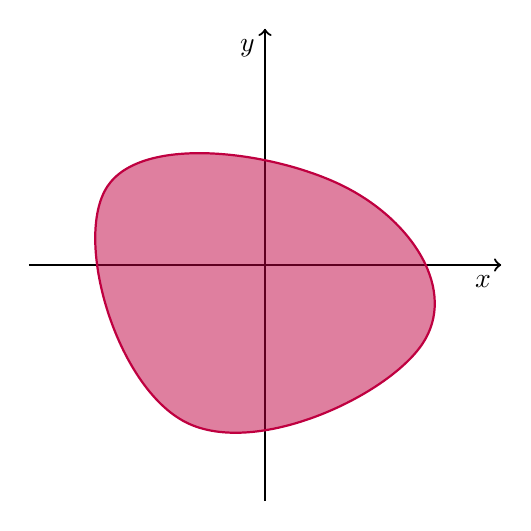
\begin{tikzpicture}[scale=1]

% Draw axes
\draw[thick,->] (-3,0) -- (3,0) node[anchor=north east]{$x$};
\draw[thick,->] (0,-3) -- (0,3) node[anchor=north east]{$y$};

% Draw shaded blob
\fill[purple, opacity=0.5] plot[smooth cycle, tension=0.8] coordinates {(-1,-2) (2,-1) (1,1) (-2,1)};
\draw[purple, thick] plot[smooth cycle, tension=0.8] coordinates {(-1,-2) (2,-1) (1,1) (-2,1)};

\end{tikzpicture}

\end{center}
\end{frame}

\begin{frame}
\frametitle{Euclid $\sim$ 300 BC}

Definition: $\pi = \frac{C}{D}$
Theorem: $A = \pi r^2$
C: circumference
D; diameter
A: area
r: radius

\end{frame}

\begin{frame}
\frametitle{Euclid's Elements - Book XII Proposition 2}

\includegraphics[clip, page=1, trim=0in 5.8in 0in 0in, width=\textwidth]{Euclid-XII-2.pdf}


{\scriptsize Source: {\tt https://mathcs.clarku.edu/\textasciitilde djoyce/java/elements/bookXII/propXII2.html}}
\end{frame}

\begin{frame}
\frametitle{Euclid's Elements - Book XII Proposition 2}

\includegraphics[clip, page=1, trim=0in 1.2in 0in 6.1in, width=\textwidth]{Euclid-XII-2.pdf}


\begin{itemize}
\item An infinite series of {\it inscribed} polygons have area approaching a limit
\item An infinite series of {\it circumscribed} polygons have area approaching a limit
\item It's the same limit
\item Then the limit must be the area of the circle
\end{itemize}

\end{frame}

\begin{frame}
\frametitle{Archimedes c. 287 BC - c. 212 BC}

Found the constant of proportionality and proved the theorem $A=\pi r^2$

\vskip 12pt

% This got GPT-4 close, then I polished it off:
%
% draw a new tikzpicture.  On the left I want a circle sliced up like a
% pie into eight equal slices.  On the right I want eight triangles of
% roughly the same size as the slices in the pie, lined up horizontally
% one right after the other.  Below the triangles draw a horizontal
% brace with "~c" below it.  To the right of the triangles draw a
% vertical brace with "~r" next to it.

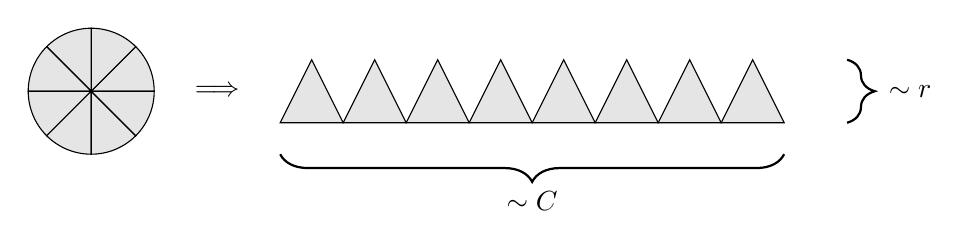
\begin{tikzpicture}[scale=0.8]

% Draw the pie
\foreach \i in {0,...,7}
{
  \draw[fill=gray!20] (0,0) -- (\i*45:1) arc (\i*45:\i*45+45:1) -- cycle;
}

\node at (2,0) {$\Longrightarrow$};

\begin{scope}[shift={(0,-0.5)}]

% Draw the triangles
\foreach \j in {0,...,7}
{
  \draw[fill=gray!20, xshift=3cm] (\j,0) -- (\j+1,0) -- (\j+0.5,1) -- cycle;
}

% Draw the braces
\draw[thick, decorate, decoration={brace, amplitude=10pt, mirror}, yshift=-0.5cm, xshift=3cm] (0,0) -- (8,0) node[midway, yshift=-0.6cm] {$\sim C$};
\draw[thick, decorate, decoration={brace, amplitude=10pt, mirror}, xshift=12cm] (0,0) -- (0,1) node[midway, xshift=0.8cm] {$\sim r$};

\end{scope}

\end{tikzpicture}

%% \[ A \approx \frac{1}{2} c r = \pi r^2 \]

\begin{center}
Definition: $\pi = \frac{C}{D}$   \qquad\qquad  Theorem: $A = \pi r^2$

\vskip 12pt

C: circumference

D: diameter

A: area

r: radius
\end{center}

\end{frame}

\begin{frame}
\frametitle{Archimedes' Method of Exhaustion}

\begin{center}
\vskip -22pt
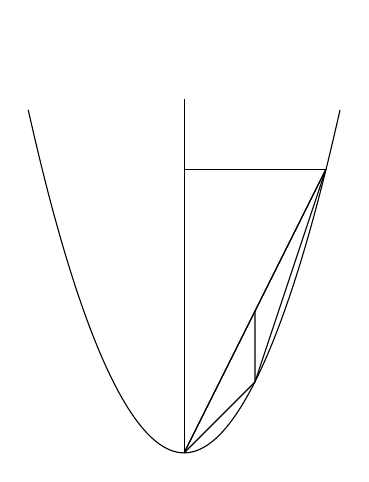
\begin{tikzpicture}[scale=0.9]

% Draw the parabola
%\draw[-] (-2,4) parabola bend (0,0) (2,4);
\draw[-] (-2.2,4.84) parabola bend (0,0) (2.2,4.84);

% y axis
\draw (0,0) -- (0,5);

\draw (0,4) -- (2,4);

\draw (0,0) -- (2,4);

\draw (0,0) -- (1,1);
\draw (1,1) -- (2,4);

% Define the points for line A
\coordinate (A) at (0,0);
\coordinate (B) at (2,4);

% Define the point (1,1)
\coordinate (P) at (1,1);

\draw[name path=line A] (A) -- (B);

% Draw the vertical line through (1,1)
\path[name path=line P] (P) -- +(0,5);

% Calculate intersection of lines
\path[name intersections={of=line A and line P, by=I}];

% Draw the line from (1,1) to the intersection point
\draw (P) -- (I);

\end{tikzpicture}

Sum of the areas of the triangles: $1 + \frac{1}{4} + \frac{1}{4^2} + \frac{1}{4^3} + \cdots$

\vskip 12pt

$x = 1 + \frac{1}{4} + \frac{1}{4^2} + \frac{1}{4^3} + \cdots  \qquad\Longrightarrow\qquad \frac{x}{4} = \frac{1}{4} + \frac{1}{4^2} + \frac{1}{4^3} + \frac{1}{4^4} + \cdots$

\vskip 12pt
$x - \frac{x}{4} = 1 \qquad\Longrightarrow\qquad x=\frac{4}{3}$

\vskip 12pt

Enclosed area of parabola = 4/3 area of inscribed triangle

\end{center}

\end{frame}

\begin{frame}
\frametitle{Cavalieri (1598-1647): Method of Indivisibles}

\tdplotsetmaincoords{70}{110}

\begin{tikzpicture}
\draw[-] (-2.2,4.84) parabola bend (0,0) (2.2,4.84);
\draw (-3,0) -- (3,0);

\foreach \i in {0,0.2,...,2.2}
{
  \draw (\i,0) -- (\i,\i^2);
}

\end{tikzpicture}%
\begin{tikzpicture}[tdplot_main_coords, line join = round, line cap = round]

% Define the main coordinates
\coordinate (O) at (0,0,0);
\coordinate (A) at (2,2,0);
\coordinate (B) at (-2,2,0);
\coordinate (C) at (-2,-2,0);
\coordinate (D) at (2,-2,0);
\coordinate (E) at (0,0,3);

% Draw the pyramid (commented out the colored base and the back side)
%\draw[fill=blue!20] (A) -- (B) -- (C) -- (D) -- cycle;
\draw (D) -- (A) -- (B);
\draw (A) -- (E);
\draw (B) -- (E);
%\draw (C) -- (E);
\draw (D) -- (E);

% Draw the slices

\foreach \i in {0.25,0.5,...,2.75}
{
   \pgfmathsetmacro\temp{(3-\i) / 3 * 2}
   % commented out the fully drawn slice
   %\draw (\temp,\temp,\i) -- (-\temp,\temp,\i) -- (-\temp,-\temp,\i) -- (\temp,-\temp,\i) -- cycle;
   \draw (\temp,-\temp,\i) -- (\temp,\temp,\i) -- (-\temp,\temp,\i);
}

\end{tikzpicture}

\[ \sum x^2 \]

\begin{center}
volume of a pyramid = $\frac{1}{3} A_b h$
\vskip 12pt
area under parabola = $\frac{1}{3} x^3$
\end{center}

\end{frame}

\begin{frame}
\frametitle{Volume of a half sphere using the method of indivisibles}

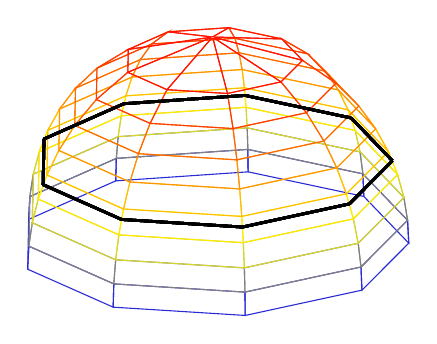
\begin{tikzpicture}
\begin{axis}[
    hide axis,
    view={40}{-30},
    samples=10
]
\addplot3 [
    mesh,
    domain=0:360,
    y domain=0:1,
] (
    {cos(x)*sqrt(1-y^2)},
    {sin(x)*sqrt(1-y^2)},
    y
);

\pgfmathsetmacro\slice{.4}

\addplot3 [
    mesh,
    domain=0:360,
    color=black,
    line width=1pt,
] (
    {cos(x)*sqrt(1-\slice^2)},
    {sin(x)*sqrt(1-\slice^2)},
    \slice
);

% \addplot3 [
%     mesh,
%     color=black,
%     samples=50,
%     domain=0:360,
%     y domain=0:.866,
% ] (
%     {cos(x)*y},
%     {sin(x)*y},
%     0.5
% );

\end{axis}
\end{tikzpicture}\qquad\qquad
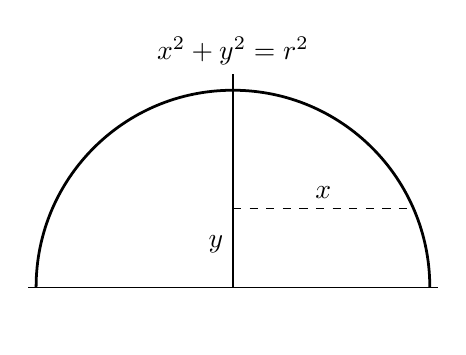
\begin{tikzpicture}[baseline={(0,-0.5)}]
\draw [line width=1pt] (2.5,0) arc (0:180:2.5);
\draw (-2.6,0) -- (2.6,0);
\draw (0,0) -- (0,2.7) node [pos=0.2, left] {$y$};
\pgfmathsetmacro\result{sqrt(2.5^2 - 1^2)}
\draw [dashed] (0,1) -- (\result,1) node [midway, above] {$x$};

\node at (0,3) {$x^2 + y^2 = r^2$};
\end{tikzpicture}

\[ \sum \pi x^2 = \sum \pi (r^2 - y^2) = \pi \sum r^2 - \pi \sum y^2 \]

\[\pi r^3 - \pi \frac{1}{3} r^3 = \frac{2}{3} \pi r^3 \]

\end{frame}

\begin{frame}
\frametitle{A Key Idea in Trigonometry}

\begin{center}
We can analyze arbitrary triangles using tools developed for right triangles

\vskip 12pt

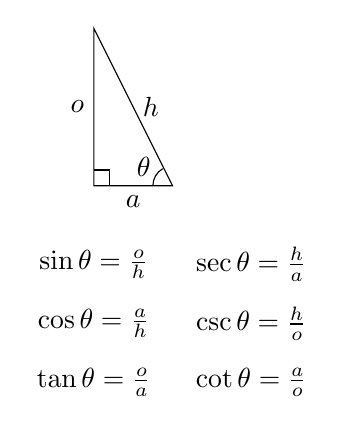
\begin{tikzpicture}
\draw (0,0) -- (1,0) node [midway, below] {$a$} -- (0,2) node [midway, right] {$h$} -- cycle node [midway, left] {$o$};
\draw (.2,0) -- (.2,.2) -- (0,.2);
\draw (1,0) ++(120:.25) arc (120:180:.25) node [pos=0.7, above left, inner sep=1pt] {$\theta$};

\node at (0,-1) {$\sin\theta = \frac{o}{h}$};
\node at (0,-1.75) {$\cos\theta = \frac{a}{h}$};
\node at (0,-2.5) {$\tan\theta = \frac{o}{a}$};

\node at (2,-1) {$\sec\theta = \frac{h}{a}$};
\node at (2,-1.75) {$\csc\theta = \frac{h}{o}$};
\node at (2,-2.5) {$\cot\theta = \frac{a}{o}$};
\end{tikzpicture}\qquad\qquad
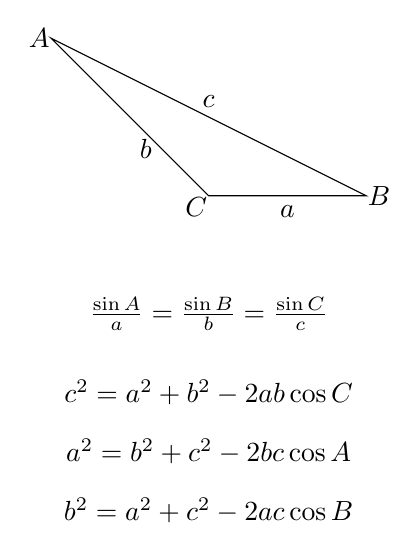
\begin{tikzpicture}[baseline={(0,-3)}]
\draw (0,0) -- (2,0) node [midway,below] {$a$} -- (-2,2) node [midway, above] {$c$} -- cycle node [pos=0.7, left] {$b$};

\node at (0,0) [below left, inner sep=0.4pt] {$C$};
\node at (2,0) [right, inner sep=0.4pt] {$B$};
\node at (-2,2) [left, inner sep=0.4pt] {$A$};

\node at (0,-1.5) {$\frac{\sin A}{a} = \frac{\sin B}{b} = \frac{\sin C}{c}$};

\node at (0,-2.5) {$c^2 = a^2 + b^2 - 2 a b \cos C$};
\node at (0,-3.25) {$a^2 = b^2 + c^2 - 2 b c \cos A$};
\node at (0,-4) {$b^2 = a^2 + c^2 - 2 a c \cos B$};
\end{tikzpicture}
\end{center}

\end{frame}

\begin{frame}
\frametitle{A Key Idea in Calculus}

\begin{center}
We can analyze plane shapes by analyzing shapes with three straight sides (left, right, bottom)
and a function defining the fourth (top) side.

\vskip 12pt

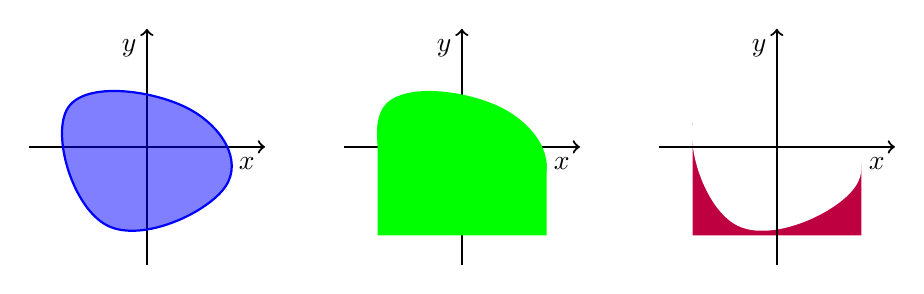
\begin{tikzpicture}[scale=0.5]

% Draw axes
\draw[thick,->] (-3,0) -- (3,0) node[anchor=north east]{$x$};
\draw[thick,->] (0,-3) -- (0,3) node[anchor=north east]{$y$};

% Draw shaded blob
\fill[blue, opacity=0.5] plot[smooth cycle, tension=0.8] coordinates {(-1,-2) (2,-1) (1,1) (-2,1)};
\draw[blue, thick] plot[smooth cycle, tension=0.8] coordinates {(-1,-2) (2,-1) (1,1) (-2,1)};

\begin{scope}[shift={(8,0)}]
% Draw axes
\draw[thick,->] (-3,0) -- (3,0) node[anchor=north east]{$x$};
\draw[thick,->] (0,-3) -- (0,3) node[anchor=north east]{$y$};

% Draw shaded blob
\fill[green] plot[smooth cycle, tension=0.8] coordinates {(-1,-2) (2,-1) (1,1) (-2,1)};
%\draw[purple] plot[smooth cycle, tension=0.8] coordinates {(-1,-2) (2,-1) (1,1) (-2,1)};
\fill [green] (-2.14,.6) -- (-2.14,-2.25) -- (2.15, -2.25) -- (2.15,-0.4);
\end{scope}

\begin{scope}[shift={(16,0)}]

% Draw shaded blob
%\draw[purple] plot[smooth cycle, tension=0.8] coordinates {(-1,-2) (2,-1) (1,1) (-2,1)};
\fill [purple] (-2.14,.6) -- (-2.14,-2.25) -- (2.15, -2.25) -- (2.15,-0.4);
\fill[white] plot[smooth cycle, tension=0.8] coordinates {(-1,-2) (2,-1) (1,1) (-2,1)};

% Draw axes
\draw[thick,->] (-3,0) -- (3,0) node[anchor=north east]{$x$};
\draw[thick,->] (0,-3) -- (0,3) node[anchor=north east]{$y$};
\end{scope}

\end{tikzpicture}

\[ A_{\rm\, blue} = A_{\rm\, green} - A_{\rm\, red} \]

\end{center}

\end{frame}

\begin{frame}
\frametitle{Another Key Idea in Calculus}

\begin{center}
We can vary the position of the right side of this region and get an ``area function''
(an indefinite integral)

\vskip 12pt

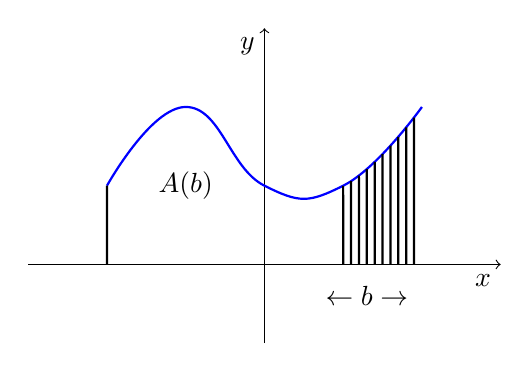
\begin{tikzpicture}

% Draw axes
\draw[->] (-3,0) -- (3,0) node[anchor=north east]{$x$};
\draw[->] (0,-1) -- (0,3) node[anchor=north east]{$y$};

    % Draw the curve and give it a name
    \draw[name path=curve, blue, thick] plot[smooth, tension=0.8] coordinates {(-2,1) (-1,2) (0,1) (1,1) (2,2)};
    % Highlight all intersection points
    \foreach \i in {-2,1,1.1,...,2}
    {
        \path[name path=line] (\i,0) -- (\i,3);
        \path[name intersections={of=curve and line, total=\t}];
        %\fill[black] (intersection-1) circle (1pt);
        \draw [thick] (\i,0) -- (intersection-1);
    }
\node at (-1,1) {$A(b)$};
\node at (1.3,-0.4) {$\leftarrow b \rightarrow$};
\end{tikzpicture}

\vskip 12pt

We couldn't do this before we restricted our attention to these straight-sided shapes.

\end{center}

\end{frame}

\begin{frame}
\frametitle{The Fundamental Theorem of Calculus}
\end{frame}

\begin{frame}
\frametitle{Berkeley, {\it The Analyst} (1734)}

\begin{quotation}
    And what are these Fluxions? The Velocities of evanescent Increments? And what are these same evanescent Increments? They are neither finite Quantities nor Quantities infinitely small, nor yet nothing. May we not call them the ghosts of departed quantities?
\end{quotation}

Mathematics historian Judith Grabiner comments, "Berkeley's criticisms of the rigor of the calculus were witty, unkind, and — with respect to the mathematical practices he was criticizing — essentially correct".[8] While his critiques of the mathematical practices were sound, his essay has been criticized on logical and philosophical grounds. 

\vskip 12pt
Source: Wikipedia, {\it The Analyst}
\end{frame}

\begin{frame}
\frametitle{Slope of a Parabola}

\noindent\smash{
\begin{tikzpicture}[scale=0.5, baseline={(0,3)}]
\draw[-] (-2.2,4.84) parabola bend (0,0) (2.2,4.84);
\draw (0,-1) -- (2,3);
\fill[black] (1,1) circle (2pt) node [right] {$x$};
\fill[black] (1.5,2) circle (2pt) node [right] {$x+h$};
\end{tikzpicture}
}


\[ \frac{(x+h)^2 - x^2}{h} \]
\[ = \frac{x^2+2hx+h^2-x^2}{h} \]
\[ = \frac{2hx+h^2}{h} = 2x + h \]

\begin{center}

Now let $h$ ``go to zero'' and we get $2x$.

\vskip 12pt

Is $h$ zero or isn't it?

\vskip 12pt

Can we divide by zero or not?
\end{center}
\end{frame}

\begin{frame}
\frametitle{Augustin-Louis Cauchy, {\it Cours D'Analyse} (1821)}

Limits

\begin{definition}[Derivative]
\[ \frac{df(x)}{dx} = \lim_{h\to 0} \frac{f(x+h) - f(x)}{h} \]
\end{definition}

\begin{definition}[Continuity]
$f(x)$ is {\it continuous} at $x_0$ if
\[ \lim_{x\to x_0} f(x) = f(x_0) \]
\end{definition}

\begin{theorem}
Polynomials are continuous everywhere.
\end{theorem}

\end{frame}

\begin{frame}
\frametitle{Slope of a Parabola with Limits}
\[ f(x) = x^2 \]

\begin{align*}
\frac{d f(x)}{dx} & = \lim_{h\to 0} \frac{f(x+h) - f(x)}{h} \quad \text{Definition of Derivative} \\
& = \lim_{h\to 0} \frac{(x+h)^2 - x^2}{h} \\
& = \lim_{h\to 0} \frac{x^2+2xh-h^2-x^2}{h} \\
& = \lim_{h\to 0} \frac{2xh-h^2}{h} \\
& = \lim_{h\to 0} (2x-h) \\
& = 2x \quad \text{by continuity of polynomials} \\
\end{align*}

\end{frame}

\begin{frame}
\frametitle{Bernhard Riemann - The Riemann Integral}
\end{frame}

\begin{frame}
\frametitle{Georg Cantor - Set Theory}

Two sets are of equal size (cardinality) if a one-to-one mapping can be set up between them.

Rational numbers have the same cardinality as the integers

Integers, rationals, tuples of integers and rationals all have the same cardinality

They are ``countable''

The real numbers are {\it not} countable.

Their cardinality in the ``continuum''
\end{frame}

\begin{frame}
\frametitle{Henri Lebesgue - ``Integral, Length, Area'' (1902)}


\end{frame}

\begin{frame}
\frametitle{Nonstandard Analysis (1960)}
\end{frame}

\begin{frame}
\frametitle{Richardson's Theorem}
\begin{mdframed}[backgroundcolor=yellow!20]
\tiny
Let $E$ be a set of expressions representing real, single valued,
partially defined functions of one real variable. $E^*$ will be the set of functions
represented by expressions in $E$.

If $A$ is an expression in $E$, $A(x)$ is the function denoted by $A$.

It is assumed that $E^*$ contains the identity function and the rational numbers as
constant functions and that $E^*$ is closed under addition, subtraction, multiplication and composition.
In every case it is also supposed that given $A$ and $B$ in $E$
there is an effective procedure for finding expressions in $E$ to represent:

$$A(x) + B(x)$$
$$A(x) - B(x)$$
$$A(x) \cdot B(x)$$
$$A(B(x))$$

$A(x) \equiv B(x)$ will mean that $A(x)$ and $B(x)$ are defined at the same points and are equal wherever they are defined.

The integration problem for $(E, E^*)$ is the problem of deciding, given $A$ in $E$,
whether there is a function $f(x)$ in $E^*$ so that $f'(x) \equiv A(x)$.

If $E^*$ satisfies conditions 1, 2, and 3, the integration problem for $(E, E^*)$ will be unsolvable.
\begin{enumerate}
\item $E^*$ contains $\ln 2$, $\pi$, $e^x$, $\sin x$.
\item There is a function, $\mu(x)$, in $E^*$ so that $\mu(x)= |x|$ for $x \ne 0$.
\item There is a totally defined function, $\mathcal{B}(x)$, in $E^*$ so that for no function, $f(x)$,
in $E^*$ and no interval $I$, is $f'(x) = \mathcal{B}(x)$ on $I$.
\end{enumerate}
Daniel Richardson,\\
{\it Some Undecidable Problems involving Elementary Functions of a Real Variable},
\\
The Journal of Symbolic Logic, Volume 33, Number 4, Dec. 1968

\end{mdframed}
\end{frame}

\begin{frame}
\frametitle{The Risch Algorithm}
\end{frame}

\begin{frame}
\frametitle{Typical University Course Sequence}
\begin{center}
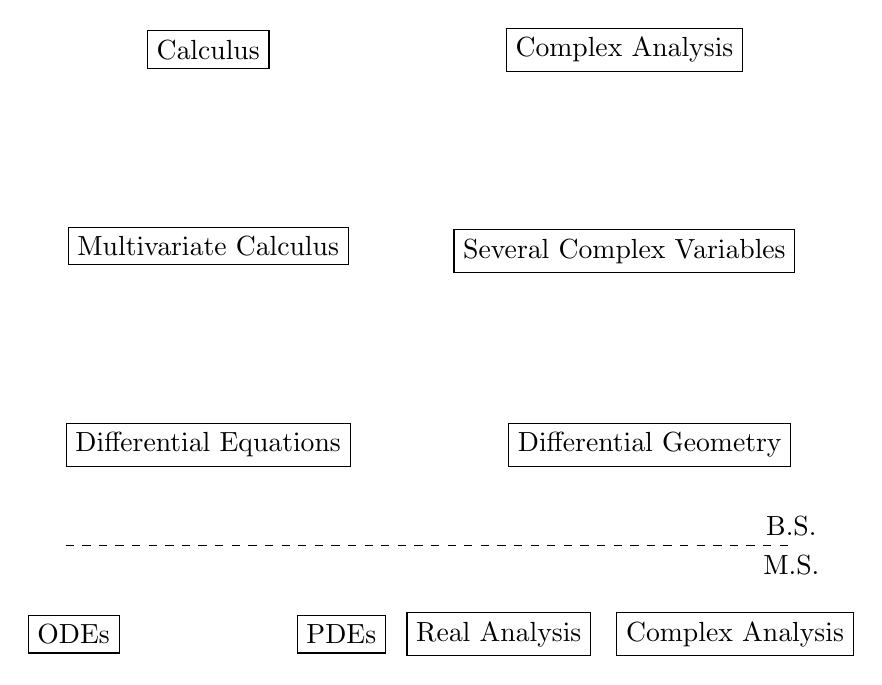
\begin{tikzpicture}[node distance=2cm]
\node [draw] (calc) {Calculus};
\node [draw, below=of calc] (mv) {Multivariate Calculus};
\node [draw, node distance=3cm, right=of calc] (ca) {Complex Analysis};
\node [draw, below=of ca] (scv) {Several Complex Variables};
\node [draw, below=of mv] (diffeq) {Differential Equations};
\node [draw, right=of diffeq] (diffgeo) {Differential Geometry};
\node [below=of diffeq] (p) {};
\node [draw, node distance=1cm, left=of p] (ode) {ODEs};
\node [draw, node distance=1cm, right=of p] (pde) {PDEs};
\node [draw, right of=pde] (real) {Real Analysis};
\node [draw, node distance=3cm, right of=real] {Complex Analysis};

% Calculate halfway point
\path (diffeq) -- node[midway] (midpoint) {} (p);

% Draw line
\draw [dashed] (diffeq.west |- midpoint) -- (diffgeo.east |- midpoint) node[below] {M.S.} node[above] {B.S.};
\end{tikzpicture}
\end{center}
\end{frame}

\begin{frame}
\frametitle{A classic multivariate ``trick''}
\[ \int_{-\infty}^{\infty} e^{-x^2} dx \]
\end{frame}

\begin{frame}
\frametitle{A classic complex analysis ``trick''}
maybe
\[ \int_{0}^{\infty} \frac{\sin x}{x} dx \]
\end{frame}

\end{document}
